\hypertarget{counting-and-discrete-probability}{%
\section{Counting and Discrete
Probability}\label{counting-and-discrete-probability}}

\hypertarget{counting}{%
\subsection{Counting}\label{counting}}

If you happen to have zero background on what we are going to talk about
in this series of topics, you might find it strange how a college course
in computer science teaches you about counting. Although this lecture is
indeed related to the concepts of cardinality, (how many things are
there), we instead go deeper into slightly more complicated ``\emph{how
many}'' questions.

\hypertarget{basic-rules-of-counting}{%
\subsubsection{Basic Rules of Counting}\label{basic-rules-of-counting}}

Counting \textbf{combinations} of related things become more
interesting. Suppose you have a two \textbf{disjoint} sets of things
called \textbf{\(A\)} and \textbf{\(B\)}, how do you count the number of
\textbf{unique combinations} of the elements of \textbf{\(A\)} and
\textbf{\(B\)}?

\hypertarget{the-product-rule}{%
\subparagraph{The Product Rule}\label{the-product-rule}}

Given a procedure with two tasks, if there are \textbf{\(n_1\)} ways to
perform the first task and \textbf{\(n_2\)} ways to perform the second
task, then there are \textbf{\(n_1 n_2\)} ways to perform the whole
procedure.

For example, let \textbf{\(A=\{a,b,c,d\}\)}, \textbf{\(B=\{x,y,z\}\)},
if you list down \textbf{all} of the \textbf{possible combinations} this
way:

\begin{longtable}[]{@{}ccccc@{}}
\toprule
& \textbf{\(a\)} & \textbf{\(b\)} & \textbf{\(c\)} & \textbf{\(d\)} \\
\midrule
\endhead
\textbf{\(x\)} & \textbf{\(ax\)} & \textbf{\(bx\)} & \textbf{\(cx\)} &
\textbf{\(dx\)} \\
\textbf{\(y\)} & \textbf{\(ay\)} & \textbf{\(by\)} & \textbf{\(cy\)} &
\textbf{\(dy\)} \\
\textbf{\(z\)} & \textbf{\(az\)} & \textbf{\(bz\)} & \textbf{\(cz\)} &
\textbf{\(dz\)} \\
\bottomrule
\end{longtable}

Since there are \textbf{\(|A|=4\)} columns and \textbf{\(|B|=3\)} rows,
then there are \textbf{\((4)(3)\)} unique combinations.

This can be generalized into \textbf{\(|S_1|=n_1\)} rows and
\textbf{\(|S_2|=n_2\)} columns. Therefore the number of unique
combinations are indeed \textbf{\(n_1 n_2\)}.

Examples

\begin{itemize}
\tightlist
\item
  How many unique plate number combinations can you produce out of the
  pattern: 3 letters and 3 numbers.
\item
  How many unique 8-bit strings can be formed
\item
  How many ways can you place 2 unique rings in your ten fingers?
\item
  How many functions are there if the domain has \textbf{\(u\)} elements
  and the range has \textbf{\(v\)} elements?
\item
  How many injective functions are there if the domain has
  \textbf{\(u\)} elements and the range has \textbf{\(v\)} elements?
\end{itemize}

As demonstrated in the first example, the product rule can be
\textbf{extended}, to not just for two tasks. For a procedure composed
of \textbf{\(m\)} tasks, \textbf{\(T_1\)}, \textbf{\(T_2\)},
\textbf{\(T_3\)}, \ldots, \textbf{\(T_m\)}, the number of ways to
perform the whole procedure is \textbf{\(n_1 n_2 n_3 \cdots n_m\)}.

Supposing you have two disjoint sets again, \textbf{\(A\)} and
\textbf{\(B\)}, how many things of either \textbf{\(A\)} or
\textbf{\(B\)} are there?

\hypertarget{sum-rule}{%
\subparagraph{Sum Rule}\label{sum-rule}}

If a task can be done \textbf{either} in one of \textbf{\(n_1\)} ways or
in \textbf{\(n_2\)} ways, (supposing each way is unique), there are
\textbf{\(n_1 + n_2\)} ways to perform the specific task.

For example let let \textbf{\(A=\{a,b,c,d\}\)},
\textbf{\(B=\{x,y,z\}\)}, the cardinality of the \textbf{\(|A \cup B|\)}
is simply \textbf{\(|A| + |B| - |A \cap B|\)}. Since \textbf{\(A\)} and
\textbf{\(B\)} are assumed to be disjoint (because each way is supposed
to be unique), then we simply add the cardinalities of the two sets
\textbf{\(A\)} and \textbf{\(B\)}.

Examples

\begin{itemize}
\tightlist
\item
  If each character of a password can either be a letter, number, or an
  underscore. How many different ways can one character be.
\item
  How many unique passwords of length 5 can you create?
\item
  How many unique passwords of length 5-8 can you create?
\end{itemize}

\begin{quote}
If we remove the assumption that the set of ways are disjoint, all we
have to do is to subtract the cardinality of their intersection.
\end{quote}

\hypertarget{subtraction-rule}{%
\subparagraph{Subtraction Rule}\label{subtraction-rule}}

If a task can be done either in one of \textbf{\(n_1\)} ways or in
\textbf{\(n_2\)} ways and there are \textbf{\(m\)} ways common between
two sets of ways, there are \textbf{\(n_1 + n_2-m\)} ways to perform the
specific task.

\begin{itemize}
\tightlist
\item
  If \textbf{\(H\)} is the set of horror movies, \textbf{\(T\)} is the
  set of thriller movies and \textbf{\(D\)} is the set of drama movies.
  How many movies are either horror, thriller, or drama?
\end{itemize}

While there is product, sum and subtraction rule, there is also a
division rule, This rule is used when some of the ways can be
categorized as one.

\hypertarget{division-rule}{%
\subparagraph{Division Rule}\label{division-rule}}

If a task can be carried out \textbf{\(n\)} ways but there are exactly
\textbf{\(d\)} identical ways for every unique way, there are
\textbf{\(\frac{n}{d}\)} unique ways.

Example

\begin{itemize}
\tightlist
\item
  How many ways can you label four corners of a square with the labels,
  \textbf{\(\{A,B,C,D\}\)}? Assuming no labels can repeat and that
  rotating the labels along the corners does not create a unique
  labelling?
\end{itemize}

\hypertarget{permutations-and-combinations}{%
\subsection{Permutations and
Combinations}\label{permutations-and-combinations}}

Some of the examples that were described in the previous sections relate
to a particular types of \textbf{counting problems}. Counting problems
like two rings on ten fingers (where you can't put two rings on the same
finger), the number of unique injections from some domain and range,
4-base pair sequences containing all 4 base pairs. These counting
problems involve counting the number of \textbf{arrangements} and
\textbf{combinations}. As it turns out problems like these have a lot of
interesting aspects:

\hypertarget{permutations}{%
\subsubsection{Permutations}\label{permutations}}

Permutation problems answer counting problems about unique arrangements.
For example:

\begin{quote}
How many ordered 3-tuples (where none of the elements repeat) can you
describe from a set of 5 objects?
\end{quote}

Since we are counting \textbf{tuples} (not subsets), the \textbf{order}
of the elements matter (i.e.~\textbf{\((a,b,c)\neq(b,a,c)\)}.

We can answer this counting problem by dividing the it into three tasks,
selecting which element resides in position 1 (5 ways, since there are 5
elements to choose from), selecting which element resides in position 2
(4 ways, since there are 4 elements to left), and selecting which
element resides in position 3 (3 ways since there are 3 elements left).
This gives the solution via product rule, \textbf{\(5(4)(3)\)}.

A \textbf{permutation} of a set of objects, is an ordered tuple (where
each element is pairwise distinct) of the objects. An
\textbf{\(r\)-permutation} on the other hand, is an ordered tuple (where
each element is pairwise district) of any size \textbf{\(r\)} subset of
the set.

For example given the set \textbf{\(S=\{a,b,c,d\}\)},
\textbf{\((a,b,c,d)\)} and \textbf{\((a,c,b,d)\)} are some permutations
of \textbf{\(S\)}. The ordered tuple \textbf{\((a,c,d)\)} is a
3-permutation of \textbf{\(S\)}, and \textbf{\((b,d)\)} is a
2-permutation of \textbf{\(S\)}.

The number of \textbf{\(r\)}-permutations of any given set with
\textbf{\(n\)} elements is denoted by \textbf{\(P(n,r)\)} or
\textbf{\(^nP_r\)}. We can derive the general formula for
\textbf{\(P(n,r)\)} using the product rule.

\begin{quote}
If \textbf{\(n\)} is a positive integer and \textbf{\(r\)} is an integer
where \textbf{\(1\leq r\leq n\)}. \[
P(n,r)=n(n-1)(n-2)\cdots(n-r+1)
\]
\end{quote}

This multiplication can actually be neatly summarized using factorials,
as shown below:

\begin{quote}
\[
\begin{aligned}
P(n,r)&=\frac{n!}{(n-r)!}\\
P(n,r)&=\frac{n(n-1)(n-2)\cdots(n-r+1)(n-r)(n-r-1)(n-r-2)\cdots(1)}{(n-r)(n-r-1)(n-r-2)\cdots(1)}
\end{aligned}
\]

The product \textbf{\((n-r)(n-r-1)(n-r-2)\cdots(1)\)} gets cancelled out
leaving:

\[
P(n,r)=n(n-1)(n-2)\cdots(n-r+1)
\]
\end{quote}

Examples:

\begin{itemize}
\tightlist
\item
  How many ways can you award the first, second and third price in
  contest with 50 participants.
\item
  How many different poker hands (5 cards) where the order matters are
  there in a deck of 52.
\end{itemize}

\hypertarget{combinations}{%
\subsubsection{Combinations}\label{combinations}}

A combination is related to a permutation but with one major difference.
While a permutation is associated to an ordered tuple, a combination is
associated to a \textbf{subset}. It answers these types of questions:

\begin{quote}
How many subsets of size 3 can you describe from a set of 5 objects?
\end{quote}

Since we are now counting subsets we need to take note that \textbf{set
equality} behaves differently. The order of the elements in a set
doesn't matter (i.e.~\textbf{\(\{a,b,c\}=\{b,a,c\}\)}).

To answer this counting problem, all we need to do is to apply the
\textbf{division} rule after calculating the number of permutations:

\begin{quote}
\[
\begin{aligned}
S&=\{a,b,c,d,e\}\\\\
\{a,b,c\}&\to\Bigg\{
  \begin{matrix}
      (a,b,c)\\
      (b,c,a)\\
      \vdots\\
      (b,a,c)\\
  \end{matrix}\\
  \end{aligned}
\]

\[
\begin{aligned}
\{b,c,d\}&\to\Bigg\{
  \begin{matrix}
      (b,c,d)\\
      (c,d,b)\\
      \vdots\\
      (d,c,b)\\
  \end{matrix}\\
  \end{aligned}
\]

\[
\begin{aligned}
  &\vdots\\
  \\
  \{c,d,e\}&\to\Bigg\{
  \begin{matrix}
      (c,d,e)\\
      (d,c,e)\\
      \vdots\\
      (e,c,d)\\
  \end{matrix}
\end{aligned}
\]
\end{quote}

Since one combination is actually equivalent to \textbf{\(P(3,3)\)}
permutations. We simply divide the total amount of 3-permutations by
\textbf{\(P(3,3)\)}. Which is \textbf{\(\frac{60}{6}=10\)} combinations.
This gives us the formula for \textbf{\(r\)-combinations} from a set of
\textbf{\(n\)} elements:

\begin{quote}
\[
\begin{aligned}
C(n,r)&=\frac{P(n,r)}{P(r,r)}\\
C(n,r)&=\frac{\frac{n!}{(n-r)!}}{\frac{r!}{(r-r)!}}\\
C(n,r)&=\frac{n!}{r!(n-r)!}
\end{aligned}
\]
\end{quote}

The number of \textbf{\(r\)} combinations in a set of \textbf{\(n\)}
elements has, is denoted as \textbf{\(C(n,r)\)}. It also usually denoted
using \textbf{\({n\choose r}\)}

Examples:

\begin{itemize}
\tightlist
\item
  In a 6/42 lottery ticket, you select a set of \textbf{\(6\)} positive
  integers from a set of \textbf{\(42\)} positive integers. How many
  unique lottery tickets are there?
\item
  Given a sorted list 6 unique numbers, how many sorted sublists are
  there
\item
  How many bit strings of length 7 are there with exactly 3 zeroes?
\item
  In the binomial expansion of \textbf{\((x+y)^3\)}, what is the
  coefficient of \textbf{\(x^2y\)}.
\end{itemize}

\hypertarget{binomial-theorem}{%
\subsubsection{Binomial Theorem}\label{binomial-theorem}}

Looking back at the previous example, we can see how we are able to use
combinatorial truths to figure out the coefficient of a term in the
expansion of the binomial \textbf{\((x+y)^3\)}. As it turns out the same
reasoning can be used for any binomial expansion \textbf{\((x+y)^n\)}.

In the following binomial, the expansion is found by adding all possible
combinations of \textbf{\(x\)}'s and \textbf{\(y\)}'s from all
\textbf{\((x+y)\)}.

\[
(x+y)^n=\underbrace{(x+y)(x+y)\cdots(x+y)}_n
\]

You can imagine one of the terms in the expansion to be of the form,

\[
cx^iy^{n-i}=cu_1u_2\cdots u_n
\]

where \textbf{\(u_i\)} is either \textbf{\(x\)} or \textbf{\(y\)} and
the coefficient \textbf{\(c\)} is the number of times the exact
combination of \textbf{\(x\)} and \textbf{\(y\)} is repeated. Therefore,
to figure out the coefficient of some arbitrary term
\textbf{\(x^iy^{n-i}\)} in the binomial expansion, you just have to
answer the combinatorial question:

\begin{quote}
how many \textbf{\(u_1u_2\cdots u_n\)} are there where there are exactly
\textbf{\(i\)} \textbf{\(x\)}'s?
\end{quote}

This asks the same question as the following combinatorial question in
the context of bit strings:

\begin{quote}
how many bit stings of length \textbf{\(n\)} are there with exactly
\textbf{\(i\)} zeroes?
\end{quote}

Which can be calculated using \textbf{\(C(n,i)\)}. Therefore, we can
formulate the general form of any binomial expansion,

\[
\begin{aligned}
(x+y)^n&=\sum_{i=0}^{n}{{n \choose i}x^iy^{n-i}}\\
(x+y)^n&={n \choose 0}y^{n}+{n \choose 1}x^1y^{n-1}+\cdots+{n \choose n}x^n
\end{aligned}
\]

\begin{quote}
For the first and the last element's \textbf{\(x^0\)} and
\textbf{\(y^0\)} are ommited.
\end{quote}

The binomial theorem can be used to algorithmically calculate the
coefficients of an expansion with really large coefficients. For example
the coefficient of the term \textbf{\(x^{21} y^{13}\)} of the binomial
\textbf{\((x+y)^{34}\)}:

\[
{34 \choose 21}x^{21}y^{13}=927983760x^{21}y^{13}
\]

The binomial theorem can answer interesting question about binomials an
combinatoric forms,

\begin{quote}
What is the sum of all coefficients in the expansion of a binomial on
the \textbf{\(n\)th} degree?
\end{quote}

This can be easily answered by calculating the following sum:

\[
\begin{aligned}
\sum_{i=0}^{n}{n \choose i}&=\sum_{i=0}^{n}{n \choose i}1^i 1^{n-i}\\
\sum_{i=0}^{n}{n \choose i}&=(1+1)^n\\
\sum_{i=0}^{n}{n \choose i}&=2^n
\end{aligned}
\]

Which actually make sense if you answer the question using the product
rule since you there are 2 ways (selecting either \textbf{\(x\)} or
\textbf{\(y\)}) in each of the \textbf{\(n\)} tasks in the whole
procedure. This also makes sense on the context of bit strings since
there are exactly \textbf{\(2^n\)} unique bit strings of length
\textbf{\(n\)}.

The binomial theorem can lead us to more interesting corollaries related
to combinatoric summations,

\[
\begin{aligned}
\sum_{i=0}^{n}{(-1)^i{n \choose i}}&=\sum_{i=0}^{n}{n \choose i}(-1)^i 1^{n-i}\\
\sum_{i=0}^{n}{(-1)^i{n \choose i}}&=(-1+1)^n\\
\sum_{i=0}^{n}{(-1)^i {n \choose i}}&=0^n=0
\end{aligned}
\]

\hypertarget{pascals-identity-and-triangle}{%
\subsubsection{Pascals Identity and
Triangle}\label{pascals-identity-and-triangle}}

One more important principle related to binomial coefficients is
\textbf{Pascal's triangle}. You may have encountered this principle in
during high school algebra but this time we are approaching it in the
context of combinatorics.

One of the most important combinatoric identities is known as
\textbf{Pascal's Identity}:

\[
{n+1 \choose r}={n \choose r-1}+{n \choose r}
\]

The identity can be proven algebraically in the following way:

\[
\begin{aligned}
{n \choose r-1}+{n \choose r}&=\frac{n!}{(r-1)!(n-(r-1))!}+\frac{n!}{r!(n-r)!}\\
&=\frac{n!}{(r-1)!(n-r+1)!}+\frac{n!}{r!(n-r)!}\\
&=\frac{n!r}{r!(n-r+1)!}+\frac{n!(n-r+1)}{r!(n-r+1)!}\\
&=\frac{n!r+n!(n-r+1)}{r!(n-r+1)!}\\
&=\frac{n!(n+1)}{r!(n+1-r)!}\\
&=\frac{(n+1)!}{r!(n+1-r)!}\\
{n \choose r-1}+{n \choose r}&={n+1 \choose r}
\end{aligned}
\]

This identity actually proves the mechanism behind Pascal's triangle

\[
\begin{array}{ccccccccccccc}
& & & & & & &1& & & & &\\
& & & & & &1& &1& & & &\\
& & & & &1& &2& &1& & &\\
& & & &1& &3& &3& &1& &\\
& & &1& &4& &6& &4& &1&\\
& &1& &5& &10& &10& &5& &1\\
&1& &6& &15& &20& &15& &6& &1
\end{array}
\]

\[
\begin{array}{ccccccccccc}
&&&&&&&{0 \choose 0}&&&&&\\
&&&&&&{0 \choose 0}&&{0 \choose 0}&&&&\\
&&&&&{2 \choose 0}&&{2 \choose 1}&&{2 \choose 2}&&&\\
&&&&{3 \choose 0}&&{3 \choose 1}&&{3 \choose 2}&&{3 \choose 3}&&\\
&&&{4 \choose 0}&&{4 \choose 1}&&{4 \choose 2}&&{4 \choose 3}&&{4 \choose 4}&\\
&&{5 \choose 0}&&{5 \choose 1}&&{5 \choose 2}&&{5 \choose 3}&&{5 \choose 4}&&{5 \choose 5}\\
&{6 \choose 0}&&{6 \choose 1}&&{6 \choose 2}&&{6 \choose 3}&&{6 \choose 4}&&{6 \choose 5}&&{6 \choose 6}
\end{array}
\]

\hypertarget{finite-probability-space}{%
\subsection{Finite Probability Space}\label{finite-probability-space}}

One of the first mathematicians to explore the concept of probability
was the French mathematician Pierre-Simon Laplace. He studied the
concept under the context of gambling. He defined the probability of an
event as the number of outcomes leading to that event, divided by the
number of possible outcomes.

Let's start this topic by discussing some key terminologies:

\begin{itemize}
\tightlist
\item
  \textbf{experiment} - in the context of probability an experiment is a
  procedure that results to exactly one outcome out of a set of possible
  outcomes.
\item
  \textbf{sample space} - we call the set of possible outcomes of a
  particular experiment its corresponding sample space
\item
  \textbf{event} - an event is a subset of the sample space
\end{itemize}

Using laplace's definition:

\begin{quote}
if \textbf{\(S\)} is a \textbf{finite} nonempty sample space of equally
likely outcomes, and \textbf{\(E\)} is an event, given that
\textbf{\(E \subset S\)}, The probability of event \textbf{\(E\)},
(denoted by \textbf{\(p(E)\)}):

\[
p(E)=\frac{|E|}{|S|}
\]
\end{quote}

The probability of an event can only be between \textbf{\(0\)} to
\textbf{\(1\)}. That is because the \textbf{\(E\)} is a subset of
\textbf{\(S\)}. Therefore, we can conclude that its cardinality is
greater than or equal to \textbf{\(0\)} and less than or equal to
\textbf{\(|S|\)} (\(0 \leq |E| \leq |S|\)).

For example, given a box that contains 3 oranges, 6 apples, and 2
bananas, what is the probability that a fruit chosen at random from the
box is an \textbf{orange}?

To answer this question, we first identify what is the sample space and
what is the event. The sample space in this experiment is the set of
eleven fruits, 3 of them are oranges and 6 of them are apples, and two
of them are bananas. The event that we are concerned with is the event
that chooses an orange. Since there are 3 oranges, the probability for
choosing an orange can be calculated as: \textbf{\(\frac{3}{11}\)}.

Examples

\begin{itemize}
\item
  Given the same scenario above, what is the probability that two fruits
  selected at random are both bananas?
\item
  What is the probability that a ticket wins the 6/49\hspace{0pt}
  lottery? Selecting a combination of 6 numbers from 1 to 49.
\item
  After uniformly shuffling the list \textbf{\([3,2,1,1,4,5]\)}, what is
  the probability that the shuffling produces a sorted list?
\end{itemize}

\hypertarget{probabilities-of-unions-of-events}{%
\paragraph{Probabilities of unions of
events}\label{probabilities-of-unions-of-events}}

If your looking for the probability that either one of two events
\textbf{\(E\)} or \textbf{\(F\)} occurs (where both \textbf{\(E\)} and
\textbf{\(F\)} are subsets of \textbf{\(S\)}), you can simply combine
the two events into one event which corresponds to their union. Since
this union is still the subset of the sample space \textbf{\(S\)}, you
can use Laplace's definition to find the probability:

\[
\begin{aligned}
    p(E \cup F) &= \frac{|E|+|F|-|E \cap F|}{|S|}\\
    &= \frac{|E|}{|S|}+\frac{|F|}{|S|}-\frac{|E \cap F|}{|S|}\\\\
    p(E \cup F) &= p(E) + p(F) + p(E \cap F)
\end{aligned}
\]

\hypertarget{probabilities-of-complements}{%
\paragraph{Probabilities of
complements}\label{probabilities-of-complements}}

If the probability of an event is known, finding the probability that
said event doesn't occur is very easy. We can leverage the fact that
since event \textbf{\(E\)} is a subset of \textbf{\(S\)}, then the set
difference \textbf{\(S-E\)} (which is also a subset of \textbf{\(S\)}),
corresponds to all events where \textbf{\(E\)} is not the outcome. That
is because \textbf{\(S-E\)} is literally the set of all outcomes that
are not \textbf{\(E\)}. This leads us to the formula for the probability
of the \textbf{complement} of an event, (denoted by
\textbf{\(p(\overline{E})\)}):

\[
\begin{aligned}
    p(\overline{E}) &= p(S-E)\\
    &=\frac{|S-E|}{|S|}\\
    &=\frac{|S|-|E|}{|S|}\\
    &=1-\frac{|E|}{|S|}\\\\
    p(\overline{E})&=1-p(E)
\end{aligned}
\]

This principle is very useful since there are times where the
\textbf{complement} of an event is much \textbf{easier} to identify than
the event itself. For example, solving for the probability of a random
8-bit string having at least one zero directly is tedious since you have
to add the probabilities for the events where the string has one zero,
two zeroes, three zeroes, and etc. If you instead identify the
complement, which is the probability that a random 8-bit string has 8
ones, (zero zeroes, or the probability not of having at least one zero):

(Given \textbf{\(E\)} as the event where the random bit string has at
least one zero)

\[
\begin{aligned}
    p(E)&=1-P(\overline{E})\\
    &=1-\frac{|\overline{E}|}{|S|}\\
    &=1-\frac{1}{2^8}\\
    &=1-\frac{1}{256}\\\\
    p(E)&=\frac{255}{256}
\end{aligned}
\]

\hypertarget{probability-theory}{%
\subsubsection{Probability theory}\label{probability-theory}}

Laplace's definition for the probability of an event in a finite sample
space assumes that all possible outcomes have \textbf{equal} likelihood
to occur. This cannot be assumed for all experiments in the \textbf{real
world} since some outcomes are actually more likely than the others. A
coin may be \textbf{biased} in such a way that outcome of flipping to
one specific side is more likely, than the other side.

The definition for probability can be generalized for finite probability
space experiments that \textbf{don't} have equally likely outcomes. This
is done by assigning a specific probability \textbf{\(p(s)\)} for each
outcome \textbf{\(s \in S\)}. The assignment of specific probabilities
can only be valid if \textbf{\(0 \leq p(s) \leq 1\)} for each outcome
\textbf{\(s\)}, and that \textbf{\(\sum_{s \in S}{p(s)}=1\)} (each
probability is within the range \textbf{\([0,1]\)}, and the sum of all
probabilities is exactly \textbf{\(1\)}). By satisfying both conditions,
an experiment is guaranteed to have exactly one outcome among the sample
space.

This definition of probability describes the function,
\textbf{\(p:S\to [0,1]\)}, known as the \textbf{probability
distribution} for the particular experiment. The correct assignment of
each probability \textbf{\(p(S)\)} should satisfy the limit:

\[
\lim_{n\to \infty}{\frac{u}{n}}=p(s)
\]

Given that after performing the experiment \textbf{\(n\)} times, the
outcome \textbf{\(s\)} occurred \textbf{\(u\)} times. For example, as
you increase the number of times you flip an unbiased coin, the ratio of
flipping heads divided by the number of flips should approach
\textbf{\(\frac{1}{2}\)}.

An example of proper assignments of probabilities look something like
this:

\begin{quote}
Given the sample space for flipping a coin, \textbf{\(S=\{H,T\}\)}:

\begin{itemize}
\tightlist
\item
  \textbf{\(p(H)=0.5001\)}
\item
  \(p(T)=0.4999\)
\end{itemize}
\end{quote}

A probability distribution such as the above which follows Laplace's
assumption of having equally likely outcomes, is called a
\textbf{uniform distribution}. This implies that a uniformly distributed
experiment will have a probability assignment
\textbf{\(p(s)=\frac{1}{n}\)} where \textbf{\(s \in S\)} and
\textbf{\(|S|=n\)}.

This then gives us a more general definition for the probability of an
event \textbf{\(E\)} as the sum of all the probabilities of the outcomes
related to event \textbf{\(E\)}.

\[
p(E)=\sum_{s \in E}{p(s)}
\]

The formula for compound probabilities remain to be true in the general
definition of probability:

\begin{itemize}
\tightlist
\item
  \textbf{\(p(E_1 \cup E_2)=p(E_1)+p(E_2)-p(E_1 \cap E_2)\)}
\item
  \textbf{\(p(\overline{E})=1-p(E)\)}
\end{itemize}

\hypertarget{conditional-probability}{%
\paragraph{Conditional Probability}\label{conditional-probability}}

Given a six-sided dice, what is the probability that the sum of two
rolls is \textbf{divisible by three}?

To answer this, all we need to do is to figure out the event that
described above. Supposing the ordered pair \textbf{\((u,v)\)}
corresponds to the outcome rolling \textbf{\(u\)} and then rolling
\textbf{\(v\)}, the event described above corresponds to the following
set: \textbf{\(\{(1,2),(2,1),(1,5),(5,1),(2,4),(4,2),(3,3)\}\)}. Since
each of the outcomes in this event have the probability
\textbf{\(\frac{1}{36}\)}, the probability that the sum of two rolls is
divisible by three is \textbf{\(\frac{7}{36}\)}.

How would the probability change, if we change the scenario, such that
the first die roll is \textbf{\(2\)}?

A modified scenario like this asks for:

``the \textbf{conditional probability} of two rolls being divisible by
three given that the first roll is 2''

A conditional probability is often denoted by \textbf{\(p(E|F)\)} where
\textbf{\(E\)} is the desired event and \textbf{\(F\)} is the assumed
event.

We can answer these probability questions by imagining a sample space
where all first dice rolls are \textbf{\(2\)},
\textbf{\(F=\{(2,1),(2,2),(2,3),(2,4),(2,5),(2,6)\}\)}. We then look at
the set of outcomes where both \textbf{\(E\)} and \textbf{\(F\)} is
satisfied (the first roll is 2 and the sum of both rolls is divisible by
three) or the set \textbf{\(E \cap F=\{(2,1),(2,4)\}\)}. This means that
the \textbf{\(E|F\)} occurs 2 out of 6 times, giving us the conditional
probability \textbf{\(p(E|F)=\frac{1}{3}\)}.

In general the formula for a conditional probability of \(E\) given
\(F\) is:

\[
p(E|F)=\frac{p(E \cap F)}{p(F)}
\]

Let's look at another example, what is the probability that the second
flip of a fair coin is heads given that the first flip is tails?

Given \textbf{\(H\)} as the event that the second flip is heads, and
\textbf{\(T\)} as the event that the first flip is tails, we solve for
\textbf{\(p(H|T)\)}:

\[
\begin{aligned}
p(H|T)&=\frac{p(H \cap T)}{p(T)}=\frac{\frac{1}{4}}{\frac{1}{2}}\\\\
p(H|T)&=\frac{1}{2}
\end{aligned}
\]

\hypertarget{independence}{%
\subparagraph{Independence}\label{independence}}

When considering conditional probabilities, the concept of probabilistic
independence often comes up. When you think about it, the outcome of the
first coin flip \textbf{does not actually affect} the outcome of the
second coin flip. Knowing the outcome of the first coin flip will not
give us any information about the outcome of the second coin flip. In
fact you can remove the first roll out of the picture and restate the
question as the following: \textbf{``\emph{what is the probability of
flipping a heads}''}. The probability of this event is exactly the same
as the probability of \textbf{\(p(H|T)\)}. Whenever
\textbf{\(p(H|T)=p(H)\)}, we can conclude that the events \textbf{\(H\)}
and \textbf{\(T\)} are \textbf{independent}. This gives us the
mathematical definition for independent events:

\begin{quote}
\textbf{\(E\)} and \textbf{\(F\)} are independent if and only if
\(p(E \cap F)=p(E)p(F)\)

\textbf{\(p(E \cap F)=p(E)p(F)\)} is just algebraic manipulation of
\textbf{\(p(E|F)=p(E)\)}.
\end{quote}

\hypertarget{bernoulli-trials-and-binomial-distributions}{%
\paragraph{Bernoulli Trials and Binomial
Distributions}\label{bernoulli-trials-and-binomial-distributions}}

Performing an experiment that can only have two outcomes (such as
flipping a coin) has a special name, it is called a \textbf{Bernoulli
trial}. Since the trial can only have two outcomes (generally called
successes and failures), we can infer that the probability of successes,
\textbf{\(p\)} and the probability of failures, \textbf{\(q\)} will sum
up to 1, (\(p+q=1\)).

Bernoulli trials are special since there are a lot of problems that can
be solved by determining the number of successes in a given amount of
mutually independent trials.

Given \textbf{\(p\)} as the probability of success and \textbf{\(q\)} as
the probability of failure in a trial, we can solve for the probability
of having \textbf{\(k\)} successes in \textbf{\(n\)} mutually
independent trials:

\begin{quote}
When \textbf{\(n\)} trials is performed, there are a total of
\textbf{\(2^n\)} possible outcomes. The number of ways exactly
\textbf{\(k\)} successes appear in \textbf{\(n\)} trials is exactly
\textbf{\(C(n,k)\)}. Since each of these ways have the probability
\textbf{\(p^k q^{n-k}\)} (because each trial is mutually exclusive we
can just multiply all probabilities). Therefore, the probability of
having exactly \textbf{\(k\)} successes is:

\[
b(k;n,p)=C(n,k)p^k q^{n-k}
\]

The probability of a observing \textbf{\(k\)} successes in
\textbf{\(n\)} mutually exclusive Bernoulli trials with probability
success \textbf{\(p\)} is denoted by \textbf{\(b(k;n,p)\)}.
\end{quote}

The probability \textbf{\(b(k;n,p)\)} as a function of \textbf{\(k\)} is
called a \textbf{binomial distribution}.

Example:

What is the probability that a randomly generated 6-bit string has
exactly 4 zeroes? (Assuming each digit is generated independently and
the outcomes 1 and 0 have the same likelihood)

\begin{quote}
Since the value of each digit in a 6-bit string is a independent from
the other digits, and a digit can only be either a 0 (success) and a 1
(failure), we can restate this as the following probability:
\textbf{\(b(4,6,0.5)\)}. Therefore, this probability is:

\[
b(4,6,0.5)=C(6,4)0.5^40.5^2=0.2345375
\]
\end{quote}

\hypertarget{bayes-theorem}{%
\paragraph{Bayes' Theorem}\label{bayes-theorem}}

One of the most powerful theorems related to probability is the Bayes'
theorem. Named after mathematician Thomas Bayes, this theorem comes up
in inferential statistics, risk analysis, machine learning, natural
language processing and many more. Bayes theorem assesses the
probability that a particular event occurs based on some evidence.

Consider the following scenario:

\begin{figure}
\centering
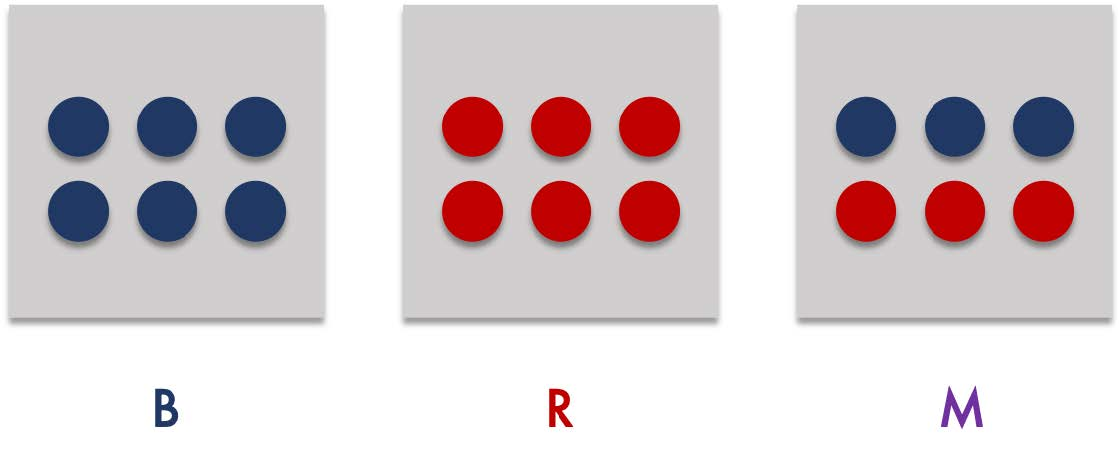
\includegraphics{https://raw.githubusercontent.com/HowDoIGitHelp/CMSC57CoursePack/master/Lecture\%20Notes/Media/counting\%20and\%20probability/bayes1.jpg}
\caption{bayes}
\end{figure}

Consider three opaque boxes, lets call them B, R, and M. Box B has 6
blue balls, box R has 6 red balls and box and box M has 3 blue balls and
3 red balls. Suppose you select a box randomly:

\begin{figure}
\centering

\includegraphics{https://raw.githubusercontent.com/HowDoIGitHelp/CMSC57CoursePack/master/Lecture\%20Notes/Media/counting\%20and\%20probability/bayes2.jpg}
\caption{bayes2}
\end{figure}

What is the probability that the selected box is box B (lets call this
\textbf{\(p(B)\))? The answer is very straightforward, since box B is
one event out of 3 possible outcomes in the sample space, the
probability is }\(\frac{1}{3}\)**. In fact the selected box is equally
likely to be box R or box M.

Suppose you pick a random ball in the selected box without looking
inside and it turned out to be a blue ball. Lets call picking a blue
ball \textbf{\(b\)}.

\begin{figure}
\centering

\includegraphics{https://raw.githubusercontent.com/HowDoIGitHelp/CMSC57CoursePack/master/Lecture\%20Notes/Media/counting\%20and\%20probability/bayes3.jpg}
\caption{bayes3}
\end{figure}

How does event \textbf{\(b\)} affect the probability that this box is
box B? Does this increase or decrease the probability that this is box
B?

This is guaranteed to not be box R since box R only has red balls. Only
half of box M's contents are blue balls while all of box B's contents
are blue balls. Because of that you can conclude the following:

\[
0=p(R|b)<p(M|b)<p(B|b)
\]

This is an example of the application of Bayesian reasoning. At the
start of the scenario, we are able to calculate that the probability of
the selected box being box B, is \textbf{\(p(B)=\frac{1}{3}\)}. We call
this probability the \textbf{prior} probability (since the probability
is before any evidence is gathered). After gathering some
\textbf{evidence} by randomly picking a ball inside the selected box
(event \textbf{\(b\)) we update our intuition about the probability of
the selected box being B. We know denote this probability as
}\(p(B|b)\)**. Which is the probability that the selected box is blue
given that one of the balls inside is blue.

What exactly is \textbf{\(p(B|b)\)}? Before we answer that, let us
derive Bayes' theorem by looking at a general scenario:

Given some event \textbf{\(Q\)}, and some evidence \textbf{\(R\)}, what
is the probability of \textbf{\(Q\)} occurring after observing the
evidence \textbf{\(R\)} (i.e.~\textbf{\(p(Q|R)\)}), if evidence
\textbf{\(R\)} occurs in \textbf{\(Q\)} with the probability
\textbf{\(p(R|Q)\)}?

We can represent this general scenario using the following diagram:

\begin{figure}
\centering
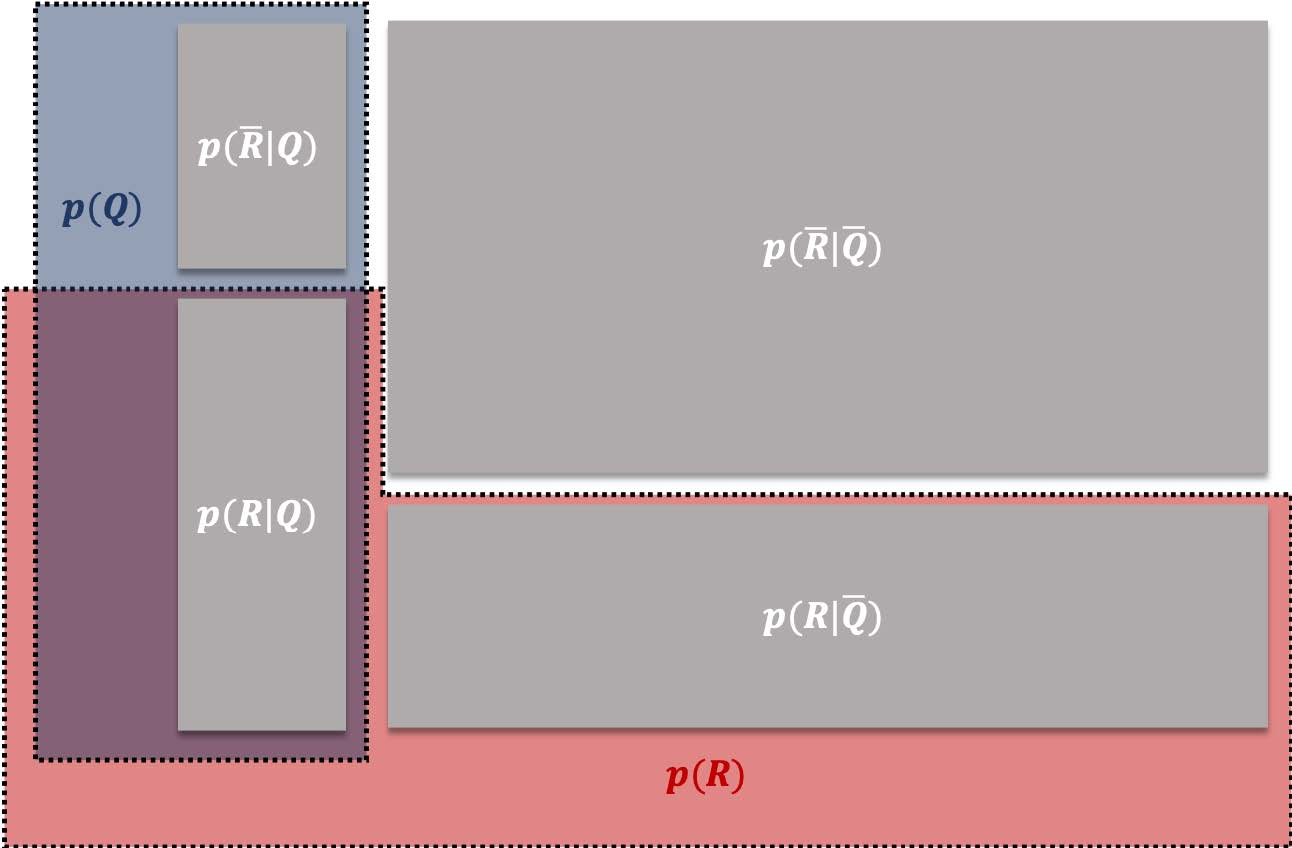
\includegraphics{https://raw.githubusercontent.com/HowDoIGitHelp/CMSC57CoursePack/master/Lecture\%20Notes/Media/counting\%20and\%20probability/bayes4.jpg}
\caption{bayes4}
\end{figure}

\[
\begin{aligned}
P(Q) &= P(R|Q) + P(\overline{R}|Q)\\
\end{aligned}
\]

This diagram represents the probabilities of all possible events in the
sample space. The sample space can be divided into two outcomes
\textbf{\(Q\)} and \textbf{\(\overline{Q}\)} (either \textbf{\(Q\)}
occurs or \textbf{\(Q\)} doesn't occur),

\begin{figure}
\centering
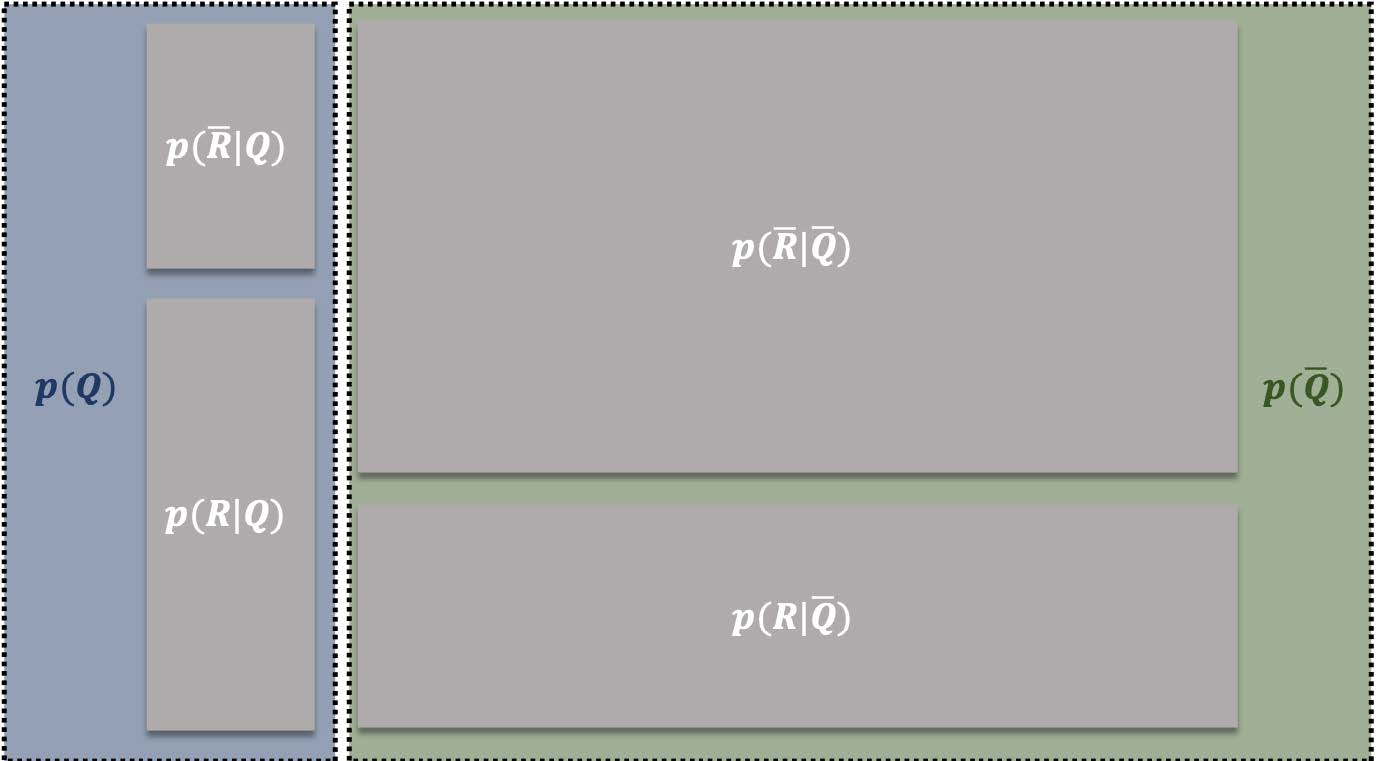
\includegraphics{https://raw.githubusercontent.com/HowDoIGitHelp/CMSC57CoursePack/master/Lecture\%20Notes/Media/counting\%20and\%20probability/bayes5.jpg}
\caption{bayes5}
\end{figure}

Within the outcome \textbf{\(p(Q)\)}, the evidence \textbf{\(R\)} has
the probability of being observed as \textbf{\(p(R|Q)\)}. Therefore to
figure out \textbf{\(p(Q|R)\)}, we just need to look at the proportion
of the occurrences of \textbf{\(R|Q\)}, among all occurrences of
\textbf{\(Q\)} in the sample space,

\begin{figure}
\centering
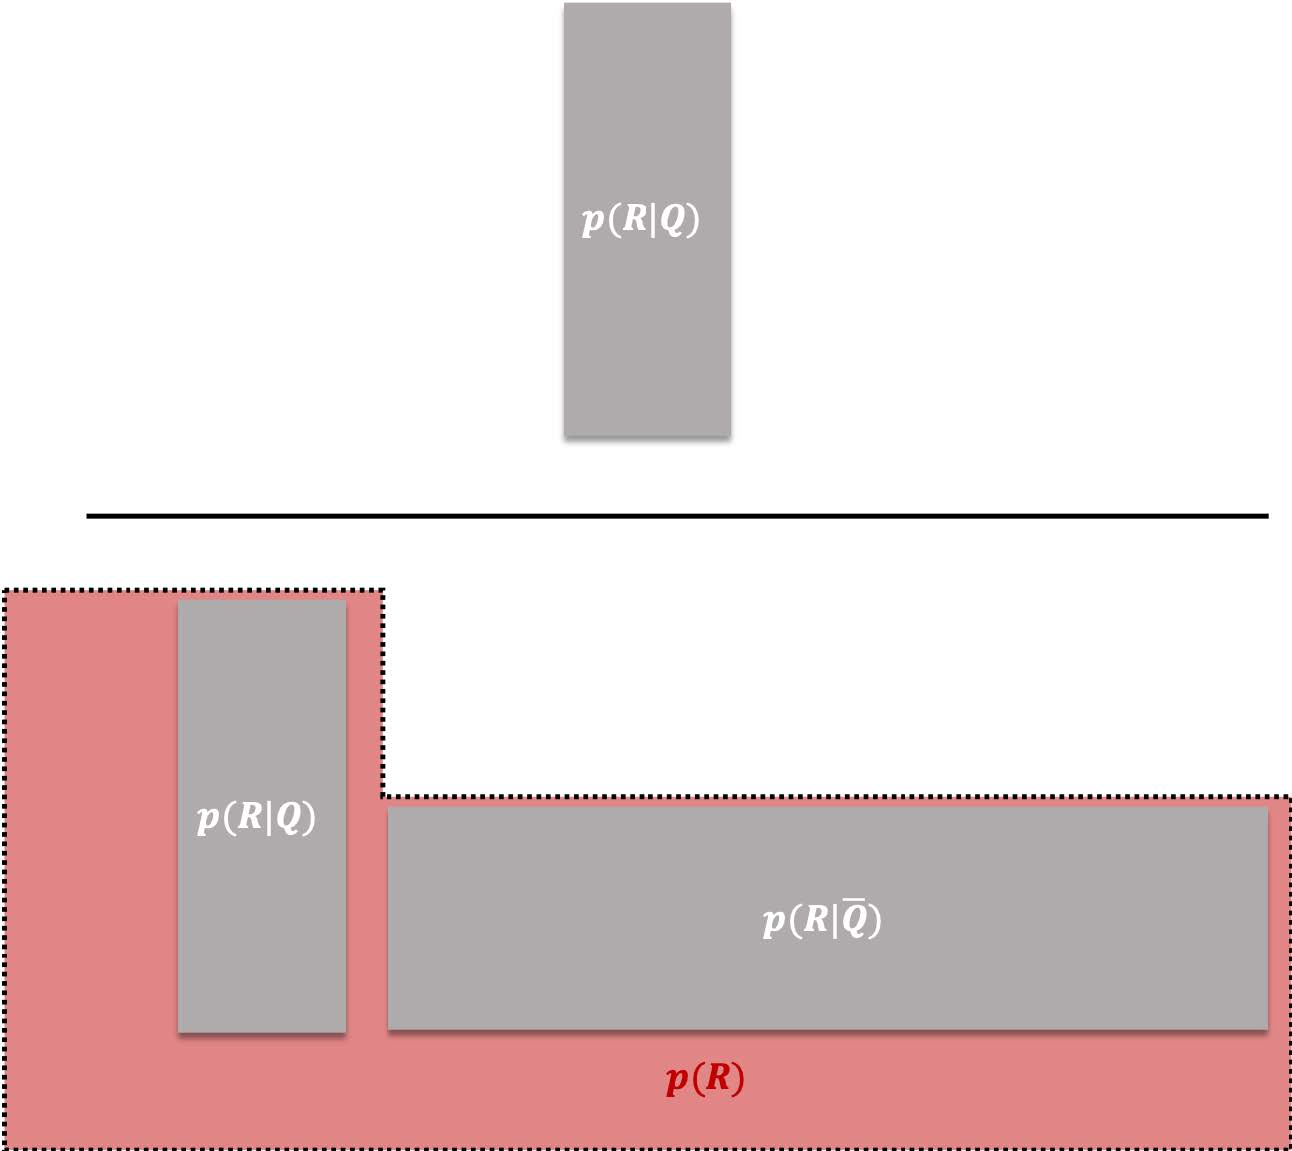
\includegraphics{https://raw.githubusercontent.com/HowDoIGitHelp/CMSC57CoursePack/master/Lecture\%20Notes/Media/counting\%20and\%20probability/bayes6.jpg}
\caption{bayes6}
\end{figure}

Suppose the size of the sample space is \textbf{\(|S|\)}, we can
represent the total number of \textbf{\(|Q|\)} occurences as
\textbf{\(p(Q)|S|\)}. That's because \textbf{\(p(Q)\)} is basically the
ratio of \textbf{\(|Q|\)} occurences divided by all possible outcomes:

\[
\begin{aligned}
p(Q)&=\frac{|Q|}{|S|}\\
p(Q)|S|&=\frac{|Q|}{|S|}|S|\\\\
p(Q)|S|&=|Q|
\end{aligned}
\]

\begin{quote}
You can think of \textbf{\(|S|\)} as the total area of the overall
rectangle and \textbf{\(p(Q)|S|\)} as the total area of the two
rectangles in the left side.
\end{quote}

Using the same reasoning we can figure out the number of occurrences
corresponding the event \textbf{\(R|Q\)}. Since there are
\textbf{\(p(Q)|S|\)} occurrences where \textbf{\(Q\)} is the outcome,
\textbf{\(p(R|Q)p(Q)|S|\)} is the number of occurrences corresponding
the event \textbf{\(R|Q\)}. Also, with the same reasoning
\textbf{\(p(R|\overline{Q})p(\overline{Q})|S|\)} is the number of
occurrences corresponding the event \textbf{\(R|\overline{Q}\)}.

Therefore, the probability \textbf{\(p(Q|R)\)} can be calculated as:

\[
\begin{aligned}
p(Q|R)=\frac{p(R|Q)p(Q)|S|}{p(R|Q)p(Q)|S|+p(R|\overline{Q})p(\overline{Q})|S|}
\end{aligned}
\]

cancelling out \textbf{\(|S|\)} on the numerator and denominator gives
us the definition of Bayes' theorem:

\[
\begin{aligned}
p(Q|R)=\frac{p(R|Q)p(Q)}{p(R|Q)p(Q)+p(R|\overline{Q})p(\overline{Q})}
\end{aligned}
\]

\begin{itemize}
\tightlist
\item
  \textbf{\(p(Q|R)\)} - the \textbf{posterior} probability, or the
  probability that Q occurs after observing evidence \textbf{\(R\)}
  occurred
\item
  \textbf{\(p(Q)\)} - the \textbf{prior} probability, or the probability
  of \textbf{\(Q\)} before observing the evidence
\item
  \textbf{\(p(R|Q)\)} - the \textbf{likelihood of the R given Q} or the
  probability of \textbf{\(R\)} occurring specifically on \textbf{\(Q\)}
  outcomes
\end{itemize}

\begin{quote}
If the general probability of the evidence \textbf{\(p(R)\)} is known,
the theorem can be written like the following:

\[
\begin{aligned}
p(Q|R)=\frac{p(R|Q)p(Q)}{p(R)}
\end{aligned}
\]
\end{quote}

To answer the question earlier, what exactly is the probability of the
selected box being the box B, given that one of the balls is blue, or
the posterior, \textbf{\(p(B|b)\)}?

\begin{itemize}
\item
  The prior probability \textbf{\(p(B)=\frac{1}{3}\)}.
\item
  The likelihood of picking blue balls in box B is
  \textbf{\(p(b|B)=1\)}.
\item
  The likelihood of picking blue balls in boxes that are not B (either R
  or M) can be calculated as,
  \textbf{\(p(b|\overline{B})=p(b|R \cup M) = \frac{p(b \cap (R \cup M))}{p(R \cup M)} = \frac{1}{4}\)}.
\end{itemize}

\begin{quote}
\textbf{\(\frac{1}{4}\)} is calculated using the following
lemma\textbf{: }\(p(b \cap (R \cup M))= p(b|R)p(R)+p(b|M)p(M)\)

The proof of this lemma, (recall conditional probability)

\[
\begin{aligned}
p(b|R)p(R)+p(b|M)p(M)&=\frac{p(b \cap R)}{p(R)}p(R)+\frac{p(b \cap M)}{p(M)}p(M)\\
&=p(b \cap R)+p(b \cap M) - 0\\
&=p(b \cap R)+p(b \cap M) - p((b \cap R) \cap (b \cap M))*\\
&=p((b \cap R) \cup p(b \cap M))\\
&=p(b \cap (R \cup  M))
\end{aligned}
\] *\(p((b \cap R) \cap (b \cap M))=0\)** because a box cannot be both R
and M at the same time, therefore there is zero probability that this
intersection of events happens. I added this so that the use of union of
events theorem is clearer.

Therefore we get \textbf{\(\frac{1}{4}\)} like this: \[
\begin{aligned}
p(b|\overline{B})&=p(b|R \cup M)\\&=\frac{p(b \cap (R \cup M))}{p(R \cup M)}\\&=\frac{p(b|R)p(R)+p(b|M)p(M)}{p(R \cup M)}\\
&=\frac{0(\frac{1}{3})+\frac{1}{2}(\frac{1}{3})}{\frac{2}{3}}\\
p(b|\overline{B})&=\frac{3}{12}=\frac{1}{4}
\end{aligned}
\]
\end{quote}

Therefore the posterior probability \textbf{\(p(B|b)\)}:

\[
\begin{aligned}
p(B|b)&=\frac{p(b|B)p(B)}{p(b|B)p(B)+p(b|\overline{B})p(\overline{B})}\\
p(B|b)&=\frac{1(\frac{1}{3})}{1(\frac{1}{3})+(\frac{1}{4})(\frac{2}{3})}\\\\
p(B|b)&=\frac{2}{3}
\end{aligned}
\]

Calculating the probabilites for other boxes supports our intuition
earlier,

\[
\begin{aligned}
p(M|b)&=\frac{p(b|M)p(M)}{p(b|M)p(M)+p(b|\overline{M})p(\overline{M})}\\
p(M|b)&=\frac{(\frac{1}{2})(\frac{1}{3})}{(\frac{1}{2})(\frac{1}{3})+(\frac{1}{2})(\frac{2}{3})}\\\\
p(M|b)&=\frac{1}{3}\\\\
p(R|b)&=\frac{p(b|R)p(R)}{p(b|R)p(R)+p(b|\overline{R})p(\overline{R})}\\
p(R|b)&=\frac{(0)(\frac{1}{3})}{(0)(\frac{1}{3})+(\frac{3}{4})(\frac{2}{3})}\\\\
p(R|b)&=0
\end{aligned}
\]

\hypertarget{bayesian-spam-filters}{%
\subparagraph{Bayesian spam filters}\label{bayesian-spam-filters}}

On of the known applications of bayesian theorems is through
probabilistic classification algorithms. The \textbf{naive bayes
algorithm} uses the bayesian theorem to classify the classification of
something based on its characteristics. This algorithm has been used in
\textbf{bayesian spam} filters where an email can be classified as spam
or not spam. Spam emails usually contain characteristic spam key words.
The presence of these spam key words on an email provide evidence for
the naive bayes algorithm that increases the likelihood for that email
to be spam. These keywords are words that are learned by the algorithm
by observing their occurences on known spam emails.

\hypertarget{random-variable-and-expected-value}{%
\paragraph{Random variable and expected
value}\label{random-variable-and-expected-value}}

The \textbf{expected value} of some random variable (some variable that
represents the outcome of an experiment) represents the most likely
value based on the probability distributions of all the possible
outcomes. Identifying the expected value answers interesting questions
about how the outcome of repeated experiments.

For example you might be interested in knowing the expected number of
heads after flipping a coin 100 times. This can be identified by
calculating the sum of all products of each outcome in the sample space
times the probability of said outcome.

Assuming the coin is fair, one coin flip has two outcomes, heads or
tails, so one coin flip can have either zero or one heads. If we imagine
a random variable \textbf{\(X\)} that represents the number of heads in
a coin flip, we know that this random variable \textbf{\(X\)} have two
possible values, \textbf{\(X=1\)} or \textbf{\(X=0\)}. Therefore the
expected value of canX be calculated as the following:

\[
\begin{aligned}
E(X)&=\sum_{s\in\{1,0\}}{p(s)s}\\
E(X)&=\frac{1}{2}(1)+\frac{1}{2}(0)\\\\
E(X)&=0.5
\end{aligned}
\]

\begin{quote}
Where \textbf{\(E(X)\)} is the expected value of \textbf{\(X\)}
\end{quote}

Meaning we expect that there are 0.5 heads in one coin flip which means
there are 0.5(100) or 50 heads in 100 coin flips.

The expected value of a random variable can be thought of as the
weighted mean value of a random variable where the weights are the
probabilities assigned to each possible value.

Expected values are very useful in more interesting experiments such as
the following example,

\emph{What is the expected value of the sum of numbers that appears in a
pair of dice?}

Since the outcome of each die is independent from the other, you can
imagine this as two repetitions of on die roll. So the expected value is
simply the expected value if one dice roll times 2:

\[
\begin{aligned}
E(X)&=\frac{1}{6}(1)+\frac{1}{6}(2)+\frac{1}{6}(3)+\frac{1}{6}(4)+\frac{1}{6}(5)+\frac{1}{6}(6)\\
E(X)&=\frac{1}{6}(21)\\
E(X)&=\frac{7}{2}\\\\
2(E(X))&=7
\end{aligned}
\]

\begin{quote}
where \textbf{\(X\)} is the random variable that represents the outcome
of a die roll.
\end{quote}

\hypertarget{variance}{%
\subparagraph{Variance}\label{variance}}

Variance measures how spread out are the possible values of a random
variable. This can be easily calculated as the the square of the
expected difference between the mean and the random variable values:

\[
\text{Var}(X)=E((X-E(X))^2)
\]

This seems like a strange formula but if you imagine the squared
difference \textbf{\((X-E(X))^2\)} as a random variable, then you can
calculate its expected value as the weighted average of squared
deviations from the mean:

\[
\text{Var}(X)=\sum_{s \in S}p(s)(s-E(X))^2
\]
